\begin{figure}[p]
\centering
    \begin{subfigure}[t]{0.45\textwidth}
    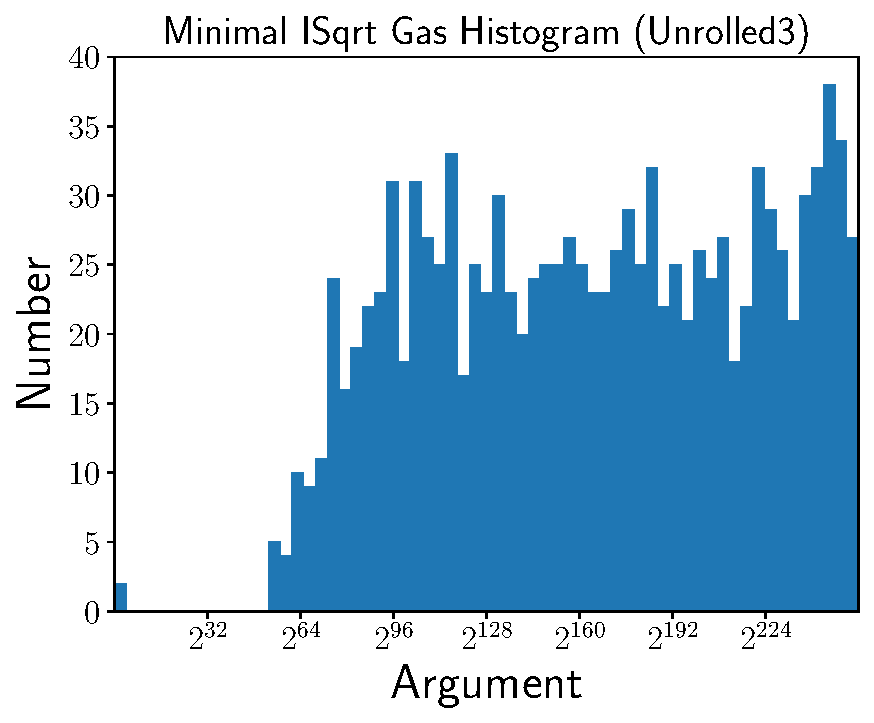
\includegraphics[width=\textwidth]{plots/minimal_hist_Unrolled3.pdf}
    \end{subfigure}
    \begin{subfigure}[t]{0.45\textwidth}
    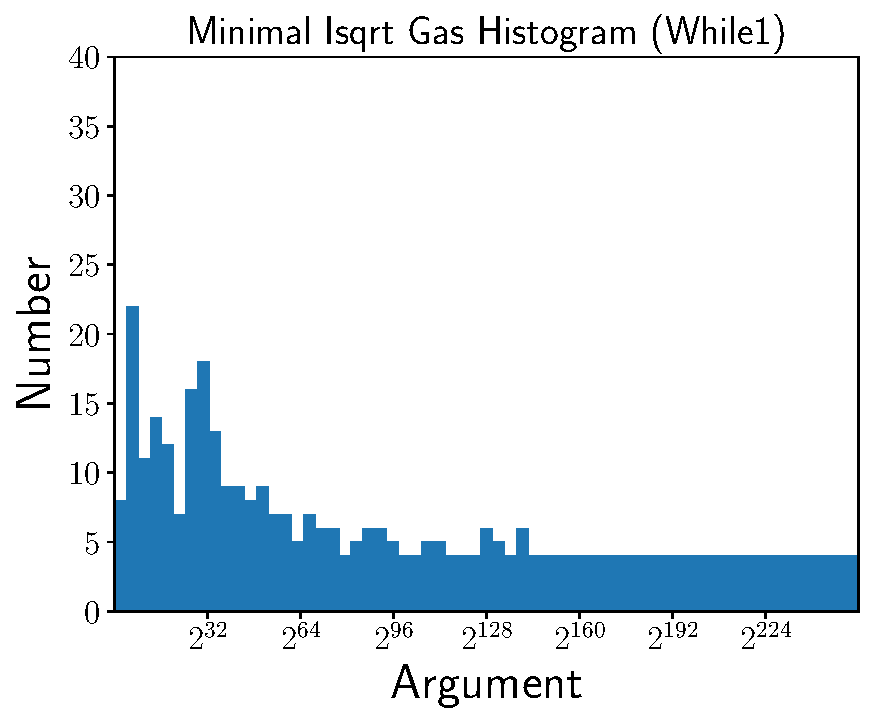
\includegraphics[width=\textwidth]{plots/minimal_hist_While1.pdf}
    \end{subfigure}

    \begin{subfigure}[t]{0.45\textwidth}
    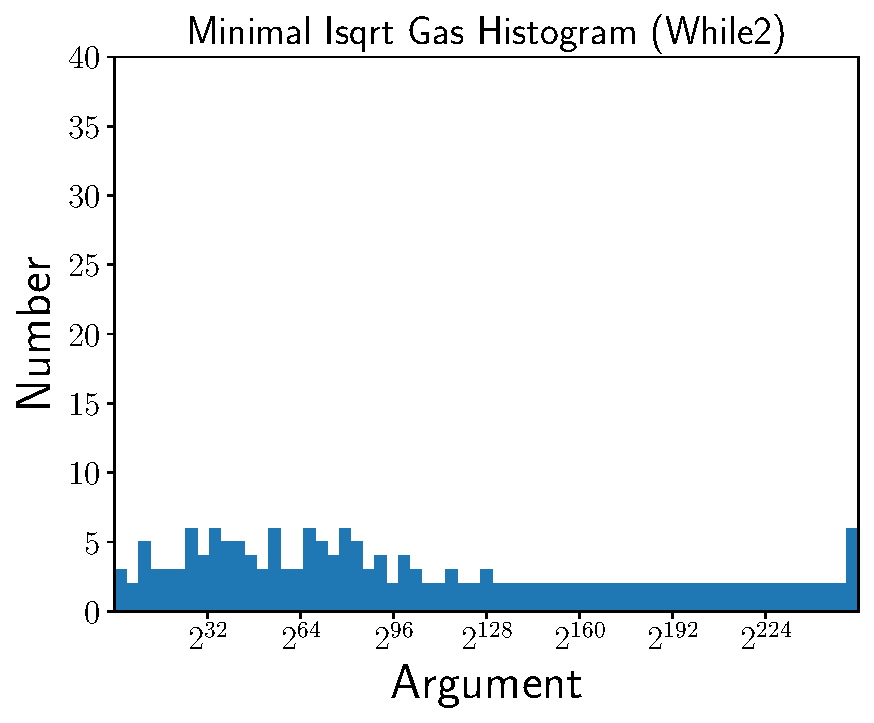
\includegraphics[width=\textwidth]{plots/minimal_hist_While2.pdf}
    \end{subfigure}
    \begin{subfigure}[t]{0.45\textwidth}
    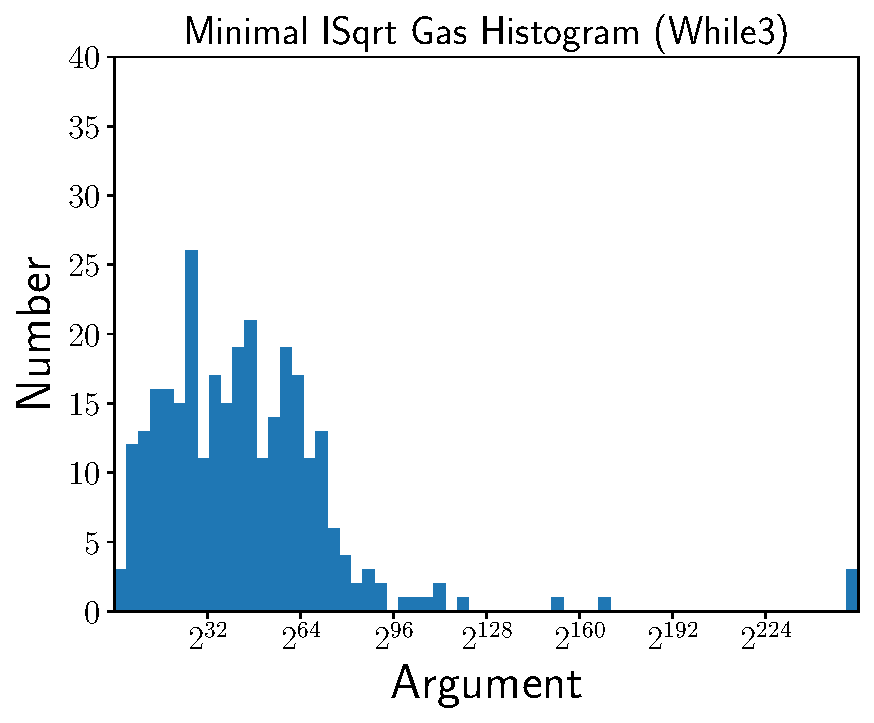
\includegraphics[width=\textwidth]{plots/minimal_hist_While3.pdf}
    \end{subfigure}
    \caption{Here we plot a histogram showing where each algorithm is minimal
        and provides more detail to the results
        in Table~\ref{table:minimal_gas_costs}.
        Each bin counts the total number instances where the algorithm's
        gas cost was minimal.
        These results are for the tests in Section~\ref{sec:comparison}.
        }
    \label{fig:minimal_gas_hist}
\end{figure}
